\begin{minipage}{\linewidth}
	\vspace{-0.5cm}
\subsection{Absenkbrunnen}
	
	\begin{itemize}
		\item Offene Wasserhaltung: kleine Bauvorhaben, geringe Absenkung
		\item Kleine Filterbrunnen: kleinere Bauvorhaben, durchlässige Böden
		\item Grosse Filterbrunnen: grosse Bauvorhaben, durchlässige Böden
		\item Wellpoint:kleine bis grosse Bauvorhaben, undurchlässige Böden (min 1.5 m Abstand zwischen Lanzen)
		
	\end{itemize}

%\end{minipage}
%
%\begin{minipage}{0.5\linewidth}
		\begin{tabular}{p{0.3\linewidth}|l|p{0.25\linewidth}}
					
			\multicolumn{3}{c|}{ \textbf{ungespannter Aquifer} } \\ \hline
			
			Vollkommener Vertikalbrunnen (Dupuit-Thiem) & $ Q = \pi \cdot k \frac{H^2 - h_0^2}{ln \frac{R}{r_0} } $	& \multirow{2}{*}{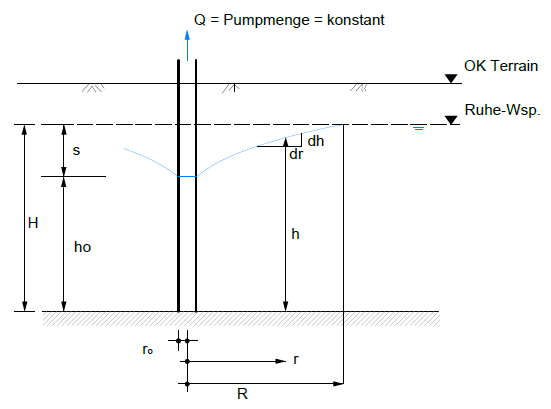
\includegraphics[width=0.8\linewidth]{images/GW9ungespAquifer.PNG}}  \\
			Filterergiebigkeit & $ v_{Grenz} \hat{\approx} \frac{\sqrt{k}}{15}$	&\\ \hline
			
			\multicolumn{3}{c|}{ \textbf{gespannter Aquifer} } \\ \hline
			
			Vollkommener Vertikalbrunnen (Dupuit-Thiem) & $ Q = 2 \cdot \pi \cdot m \cdot k \frac{H - h_0}{ln \frac{R}{r_0} } $	& \smallskip 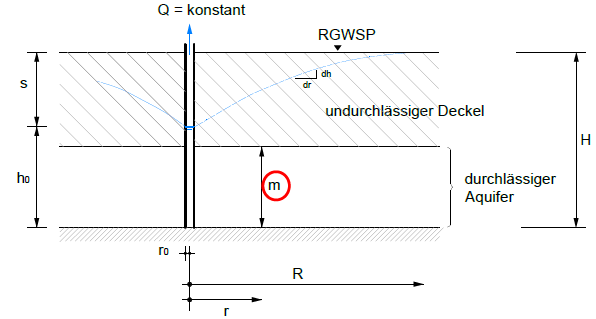
\includegraphics[width=0.8\linewidth]{images/GW10gespAquifer.PNG}  \\ \hline
			
			Unvollkommener Vertikalbrunnen (der Brunnen reicht nicht bis zur undurchlässigen Stauschicht)	& $ Q_{unvollk} \approx (1.1 \div 1.3) \cdot Q_{vollk} (H = H_1) $	& \smallskip 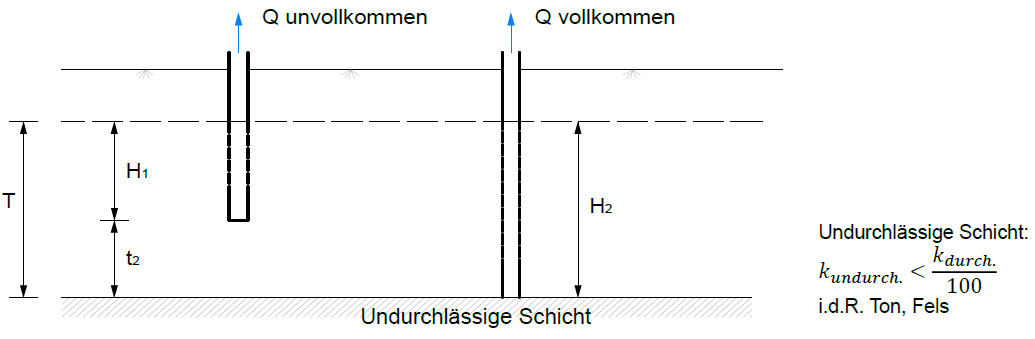
\includegraphics[width=\linewidth]{images/GW11gespAquiferunvollk.PNG}  \\
						
		\end{tabular}
	\end{minipage}
	\begin{minipage}{\linewidth}
		
		\subsubsection{Weitere Grundwasseranwendungen}
		
		\begin{tabular}{p{0.2\linewidth}|p{0.4\linewidth}|p{0.3\linewidth}}
			Bemerkung 		& Formel			&	Einheit \\ \hline
			
			Zufluss zu Bach (ungespannt) & $ Q = k \frac{H^2 - L^2}{r \cdot R} $	& \smallskip 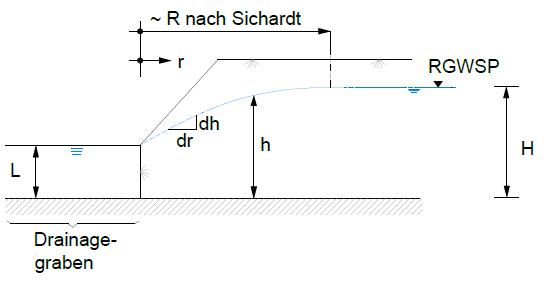
\includegraphics[width=\linewidth]{images/GW12Bachungespannt.PNG}  \\ \hline
			
			Zufluss zu Bach (gespannt)	& $ Q = m \cdot k \frac{H - L}{R} $ & \smallskip 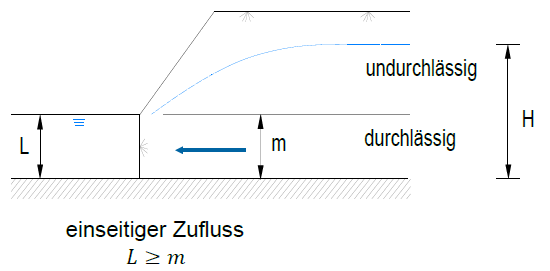
\includegraphics[width=\linewidth]{images/GW13Bachgespannt.PNG}  \\ \hline
			
			GW-Absenkung für Baugrube mit mehreren Brunnen 	& 1. Fiktiver Radius R$_A = \sqrt{\frac{a \cdot b}{\pi} } $ [m]	& R$_A$ : fiktiver Radius (Baugrubenabmessung a x b) $ R_A = \sqrt{ \frac{a \cdot b }{\pi} } $ \\
															& 2. Abschätzung Pumpwassermenge Q$_{tot} =\pi \cdot k \frac{H^2 - h^2}{ln(R) - ln(R_A) } $ [$ \frac{m^3}{s} $]												& \smallskip \multirow{7}{*}{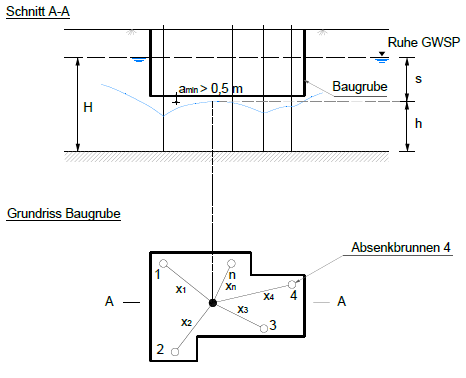
\includegraphics[width=\linewidth]{images/GW14mehrereBrunnen.PNG} }  \\
															& 3. v$_{Grenz} = \frac{ \sqrt{k} }{15} $ [$ \frac{m}{s} $]		& \\
															& 4. erf. benetzte Brunnenmantelfläche $ M_{erf} = \frac{Q_{tot} }{v_{Grenz} } [m^2]$ & \\
															& 5. Filterhöhe $ h = \frac{M_{erf} }{U_{Brunnen} } $ [m] $ \rightarrow $ Faktor 2 Sicherheit bei Anzahl Brunnen												& \\
															& 6. GW-Spiegelhöhe z an beliebiger Stelle $ z = \sqrt{ H^2 - \frac{Q_{tot} }{\pi \cdot k} [ln(R) - \frac{1}{n} ln(x_i) ] } $								& \\
															& 7. Pumpwassermenge an beliebiger Stelle Q$_{f} = \pi \cdot k \frac{H^2 - z^2 }{ln(R) - \frac{1}{n} ln(x_1 \cdot x_2 \cdot ... x_n) } $					& \\
															& 8. Pumpwassermenge pro Brunnen Q$_{erf} = \frac{Q_f}{n} $		& \\
%			\begin{enumerate}
%				\item Fiktiver Radius R$_A = \sqrt{\frac{a \cdot b}{\pi} } $ [m]
%				\item Abschätzung Pumpwassermenge Q$_{tot} =\pi \cdot k \frac{H^2 - h^2}{ln(R) - ln(R_A) } $ [$ \frac{m^3}{s} $]
%				\item v$_{Grenz} = \frac{ \sqrt{k} }{15} $ [$ \frac{m}{s} $]
%				\item erf. benetzte Brunnenmantelfläche $ M_{erf} = \frac{Q_{tot} }{v_{Grenz} } [m^2]$
%				\item Filterhöhe $ h = \frac{M_{erf} }{U_{Brunnen} } $ [m] $ \rightarrow $ Faktor 2 Sicherheit bei Anzahl Brunnen
%				\item GW-Spiegelhöhe z an beliebiger Stelle $ z = \sqrt{ H^2 - \frac{Q_{tot} }{\pi \cdot k} [ln(R) - \frac{1}{n} ln(x_i) ] } $
%				\item Pumpwassermenge an beliebiger Stelle Q$_{f} = \pi \cdot k \frac{H^2 - z^2 }{ln(R) - \frac{1}{n} ln(x_1 \cdot x_2 \cdot ... x_n) } $
%				\item Pumpwassermenge pro Brunnen Q$_{erf} = \frac{Q_f}{n} $
%			\end{enumerate}
%		& R$_A$ : fiktiver Radius (Baugrubenabmessung a x b) $ R_A = \sqrt{ \frac{a \cdot b }{\pi} } $ \\
%							&					& \smallskip 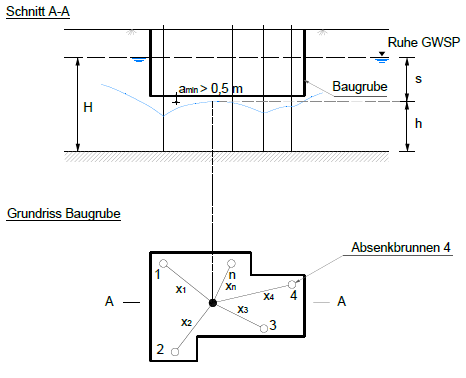
\includegraphics[width=\linewidth]{images/GW14mehrereBrunnen.PNG}  \\ \hline
			
		\end{tabular}
	\end{minipage}